% !TeX root = ../main.tex

%%% Tables %%%

\begin{table}
\centering
\caption{Accuracies and run times for all models. All reported values are averages, and $\pm$ refers to the standard deviation.}
\begin{tabular}{ccccccc}
Model       & \multicolumn{1}{c}{Training Time (Minutes)} & \multicolumn{1}{c}{Dive Accuracy} & \multicolumn{1}{c}{Subdive Accuracy}  \\ \hline
CarHMM-DFT  & $15.74 \pm 2.46$                            & -------------                     & $1.00 \pm 0.00$                       \\ 
HHMM-DFT    & $82.43 \pm 11.48$                           & $0.94 \pm 0.02$                   & $1.00 \pm 0.00$                       \\
CarHHMM     & $70.85 \pm 15.89$                           & $0.91 \pm 0.03$                   & $0.89 \pm 0.02$                       \\
CarHHMM-DFT & $81.22 \pm 16.10$                           & $0.94 \pm 0.02$                   & $1.00 \pm 0.00$                       \\
\end{tabular}
\label{table:accuracy}
\end{table}

\begin{table}[ht]
    \centering
    \caption{Estimates and standard errors of emission parameters for killer whale data.}
    \scalebox{0.8}{
    \begin{tabular}{ccccc}
    \multirow{2}{*}{Feature}                 & \multirow{2}{*}{Dive / Sub-dive Type} & \multicolumn{3}{c}{Parameter Estimate}              \\
                                             &                                      & $\hat \mu$      & $\hat \sigma$   & $\hat \phi$     \\ \hline
    \multirow{2}{*}{Dive Duration $(s)$ - $Y$} & 1                                    & $27.23 \pm 0.63$ & $10.89 \pm 0.56$ & ---             \\
                                             & 2                                    & $127.96 \pm 11.50$ & $64.13 \pm 9.21$ & ---             \\ \hline
    \multirow{3}{*}{x-acceleration $(m/s^2)$ - $\left(\mathbf{Z}^{*(1)}\right)_x$}            & 1                                    & $0.98 \pm 0.07$ & $0.04 \pm 0.00$ & $0.99 \pm 0.00$ \\
                                             & 2                                    & $0.22 \pm 0.01$ & $0.08 \pm 0.00$ & $0.87 \pm 0.01$ \\
                                             & 3                                    & $0.23 \pm 0.03$ & $0.28 \pm 0.01$ & $0.62 \pm 0.03$ \\ \hline
    \multirow{3}{*}{y-acceleration $(m/s^2)$ - $\left(\mathbf{Z}^{*(1)}\right)_y$}            & 1                                    & $0.61 \pm 0.09$ & $0.05 \pm 0.00$ & $0.99 \pm 0.00$ \\
                                             & 2                                    & $0.43 \pm 0.01$ & $0.09 \pm 0.00$ & $0.87 \pm 0.01$ \\
                                             & 3                                    & $0.38 \pm 0.04$ & $0.35 \pm 0.01$ & $0.62 \pm 0.04$ \\ \hline
    \multirow{3}{*}{z-acceleration $(m/s^2)$ - $\left(\mathbf{Z}^{*(1)}\right)_z$}            & 1                                    & $-1.00 \pm 0.11$ & $0.05 \pm 0.00$ & $0.99 \pm 0.00$ \\
                                             & 2                                    & $-0.57 \pm 0.01$ & $0.10 \pm 0.00$ & $0.87 \pm 0.01$ \\
                                             & 3                                    & $-0.35 \pm 0.04$ & $0.34 \pm 0.01$ & $0.62 \pm 0.04$ \\ \hline
    \multirow{3}{*}{Fourier sum - $Z^{*(2)}$}              & 1                                    & $27.16 \pm 0.32$ & $16.67 \pm 0.32$ & ---             \\
                                             & 2                                    & $406.98 \pm 4.42$ & $438.09 \pm 5.49$ & ---             \\
                                             & 3                                    & $9688.54 \pm 221.95$ & $14584.02 \pm 358.40$ & ---             \\ \hline
    \end{tabular}
    }
    \label{table:emis_dists}
\end{table}

%%% model definitions %%%

\begin{figure}[ht]
    \begin{subfigure}{\textwidth}
      \centering
      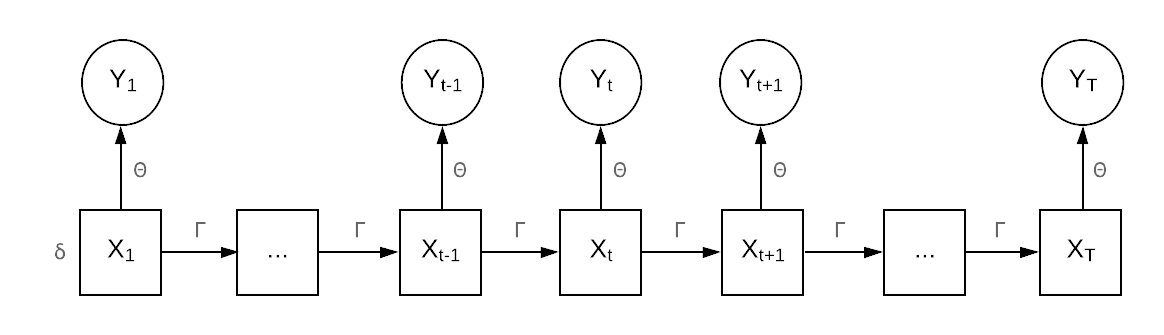
\includegraphics[width=4in]{../Plots/HMM.png}  
      \caption{Hidden Markov Model (\textbf{HMM})}
      \label{fig:HMM}
    \end{subfigure}
    %
    \newline
    %
    \begin{subfigure}{\textwidth}
      \centering
      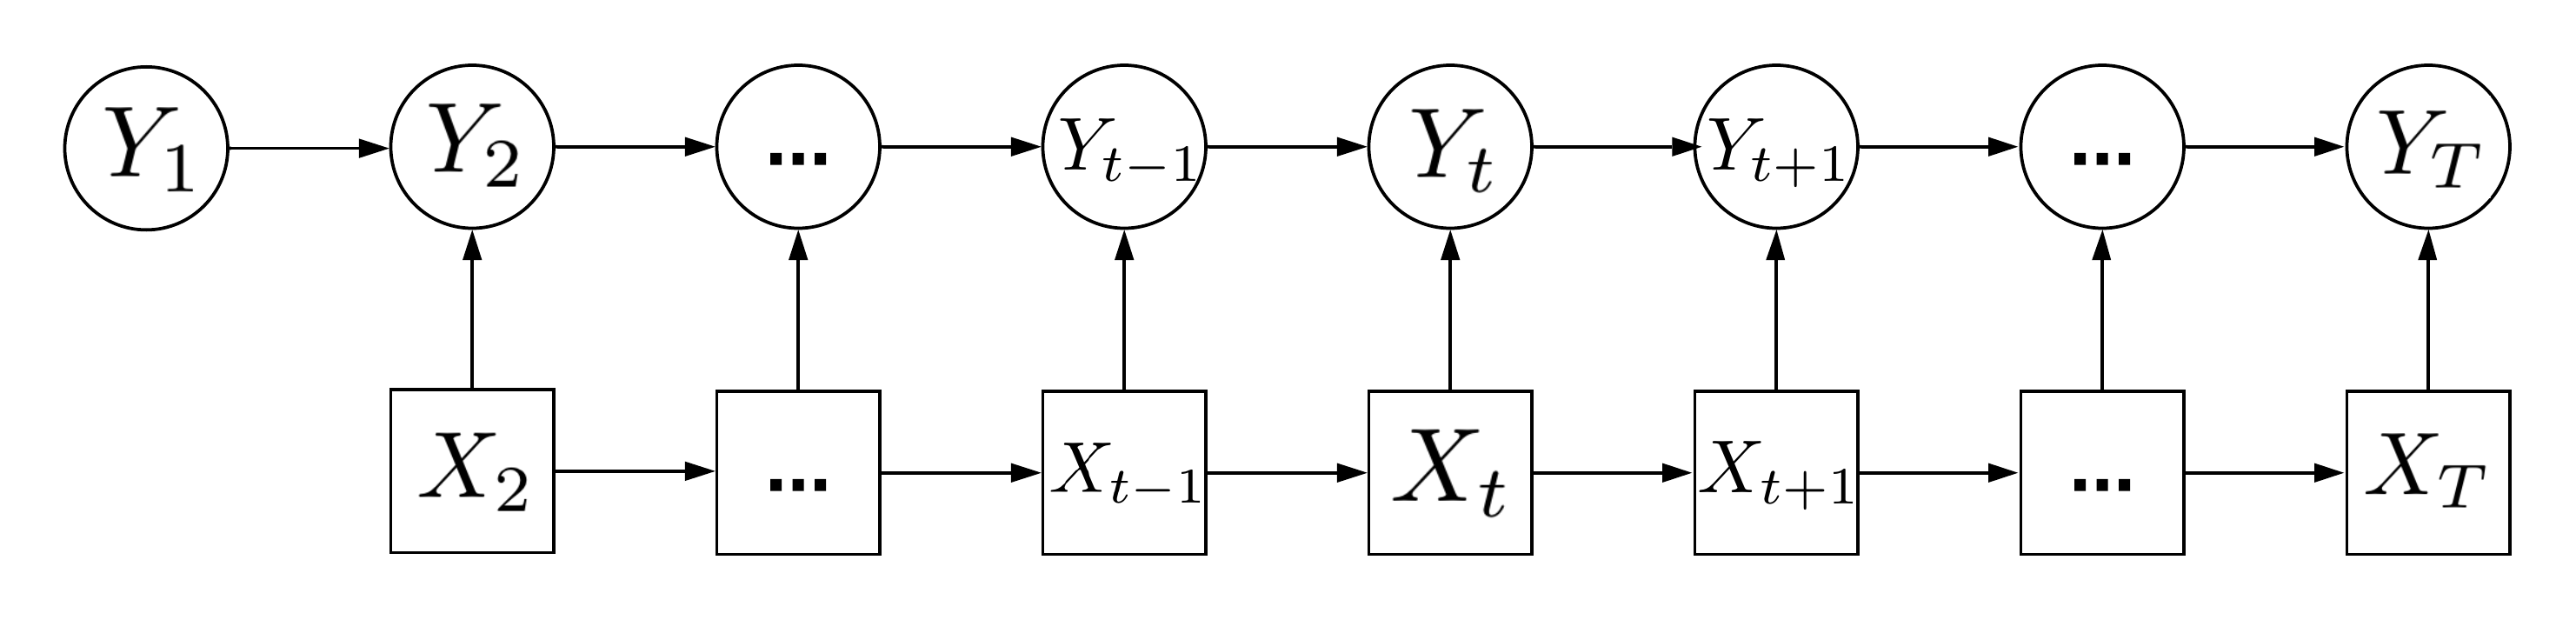
\includegraphics[width=4in]{../Plots/CarHMM.png}  
      \caption{Conditionally Auto-regressive HMM (\textbf{CarHMM})}
      \label{fig:CarHMM}
    \end{subfigure}
    %
    \newline
    %
    \begin{subfigure}{\textwidth}
      \centering
      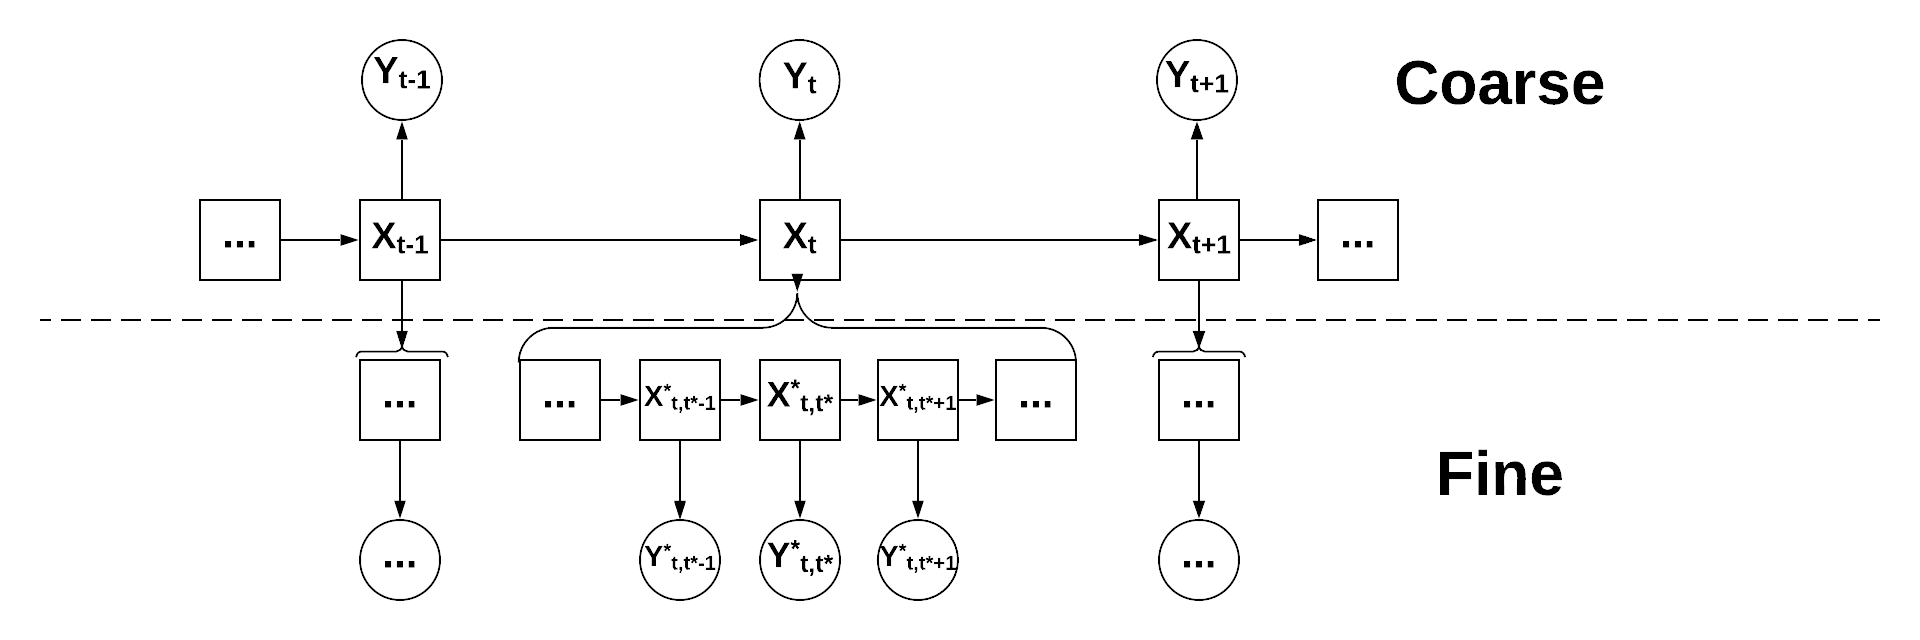
\includegraphics[width=4in]{../Plots/HHMM.png}  
      \caption{Hierarchical HMM (\textbf{HHMM})}
      \label{fig:HHMM}
    \end{subfigure}
    %
    \newline
    %
    \begin{subfigure}{\textwidth}
      \centering
      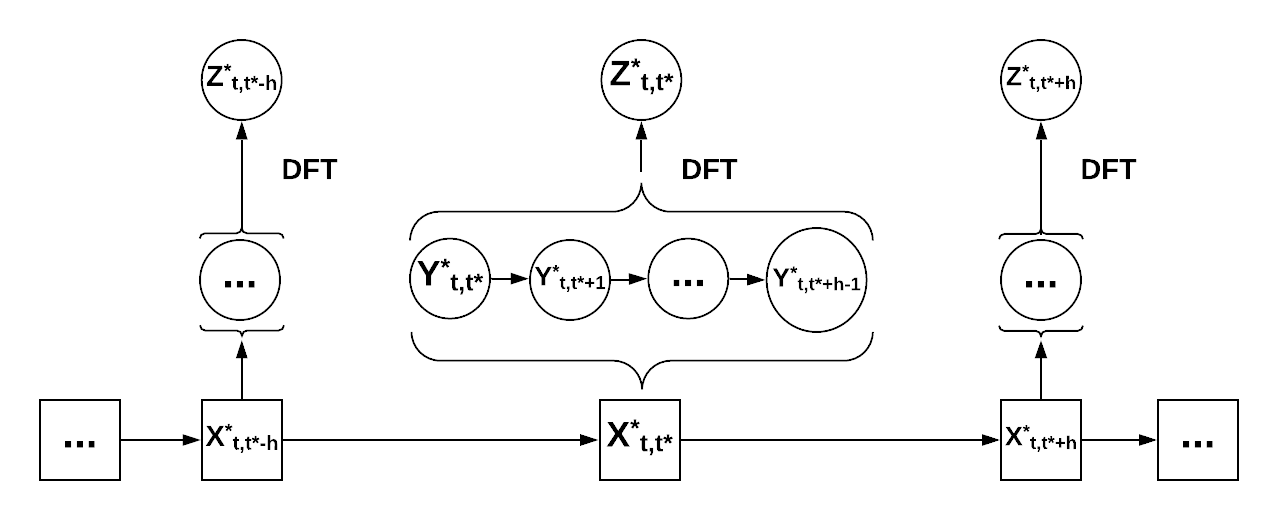
\includegraphics[width=4in]{../Plots/HMM-DFT.png}  
      \caption{HMM with Discrete Fourier Transform (\textbf{HMM-DFT})}
      \label{fig:HMM-DFT}
    \end{subfigure}
    \caption{Graphical representations of HMM models}
    \label{fig:models}
\end{figure}

%%% simulation study %%%

\begin{figure}[ht]
	\centering
	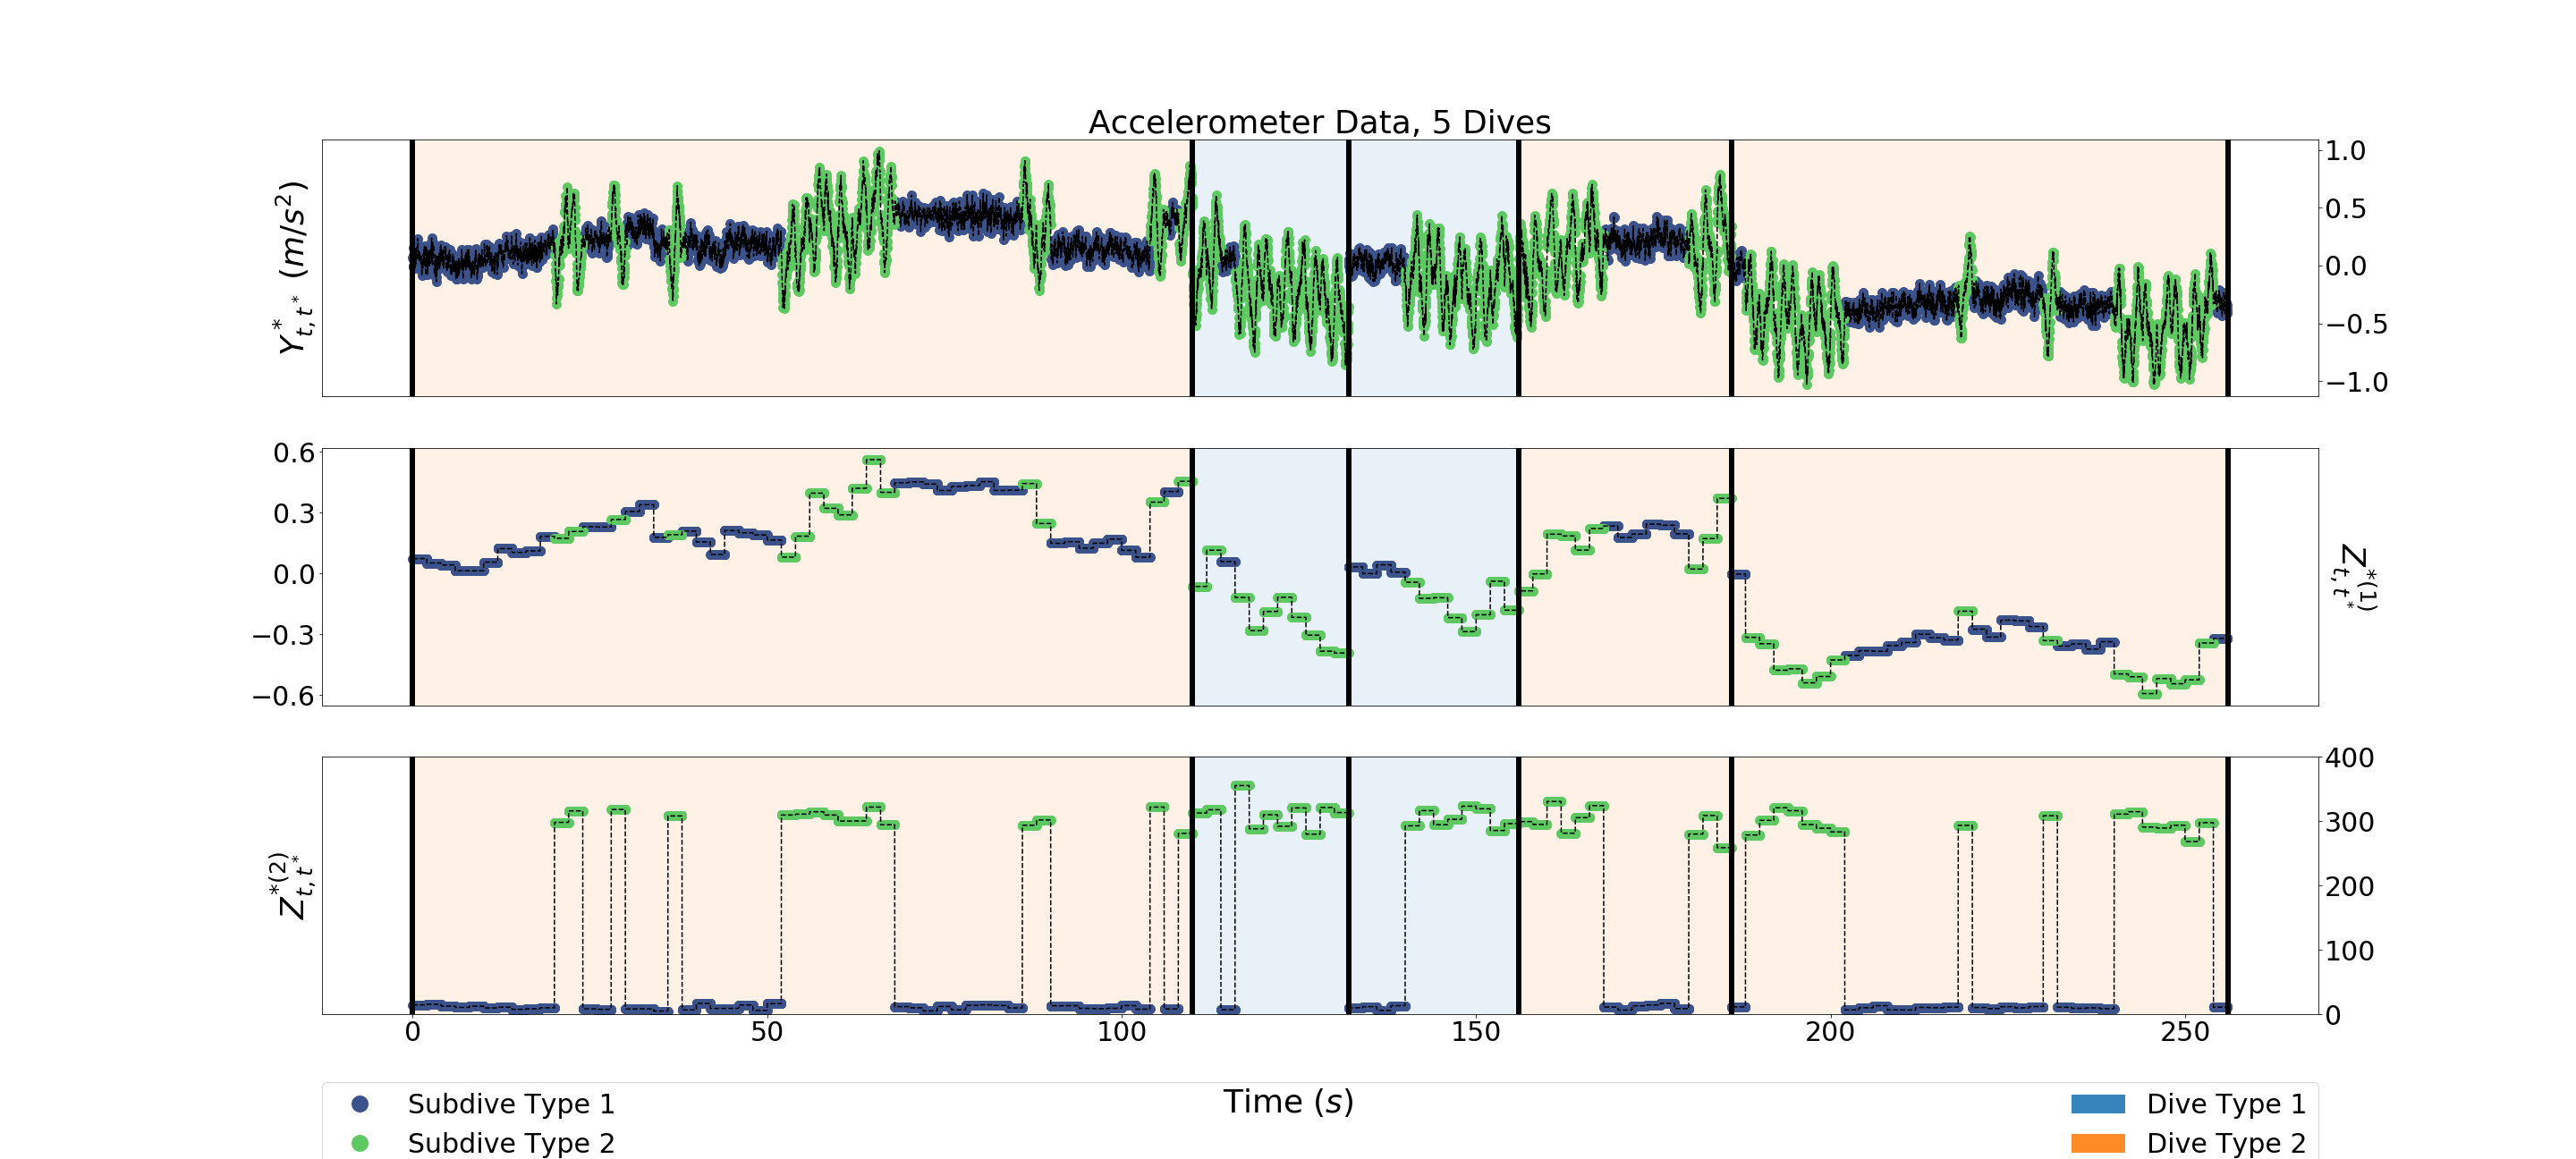
\includegraphics[width=5in]{../Plots/sim_data.png}
	\caption{Simulated acceleration data for one dive. The color of the line corresponds to the true fine-scale state of the sub-dive process, while the color of the background corresponds to the true dive type of the simulated whale.}
	\label{fig:sim_data}
\end{figure}

\begin{figure}[ht]
	\centering
	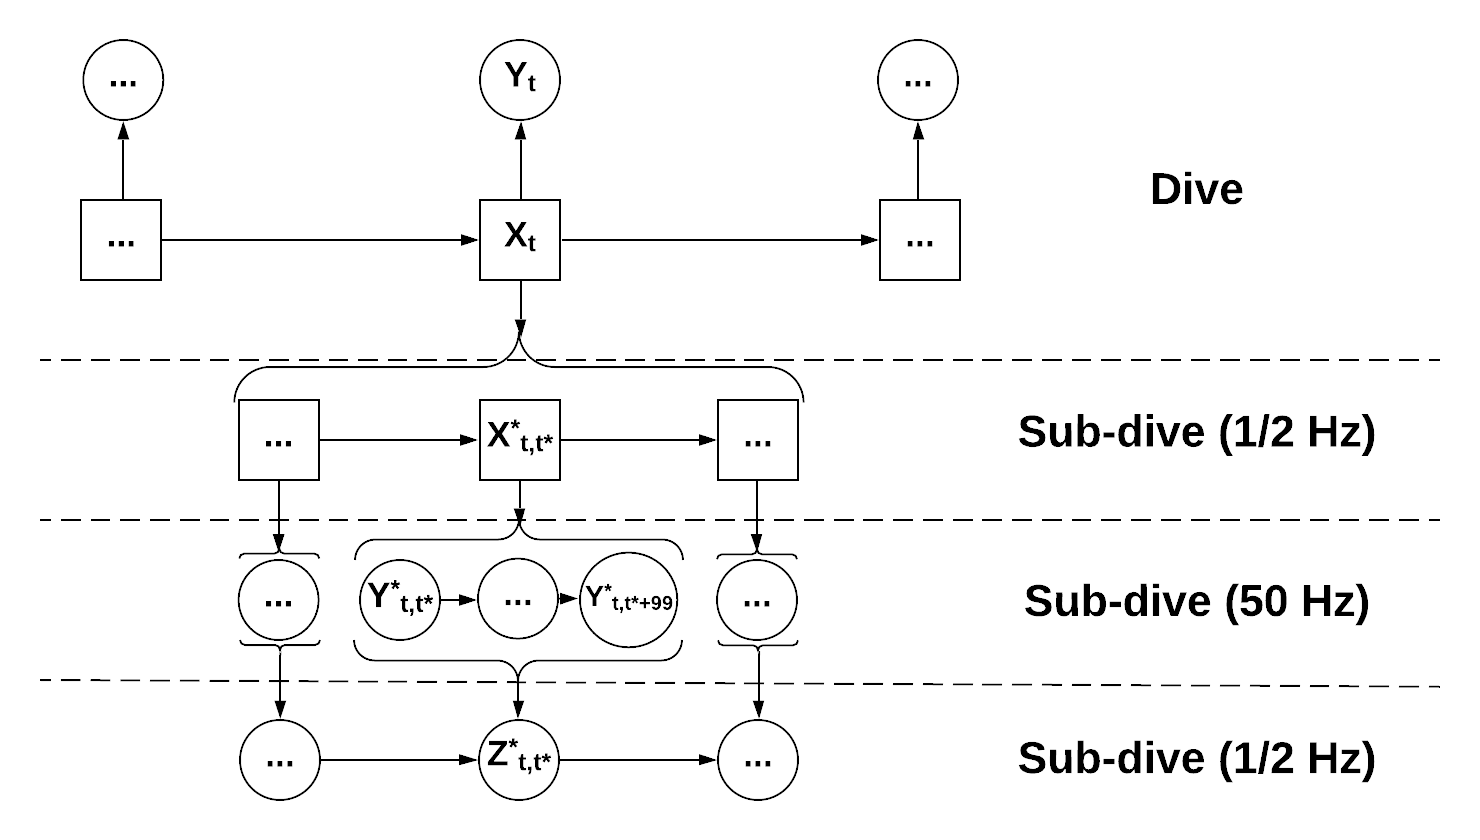
\includegraphics[width=5in]{../Plots/CarHHMM-DFT.png}
	\caption{Graphical representation the model used in the simulation and case study, the \textbf{CarHHMM-DFT}.}
	\label{fig:CarHHMM-DFT}
\end{figure}

\begin{figure}[ht]
    \centering
    \begin{subfigure}[t]{1.0\textwidth}
        \centering
        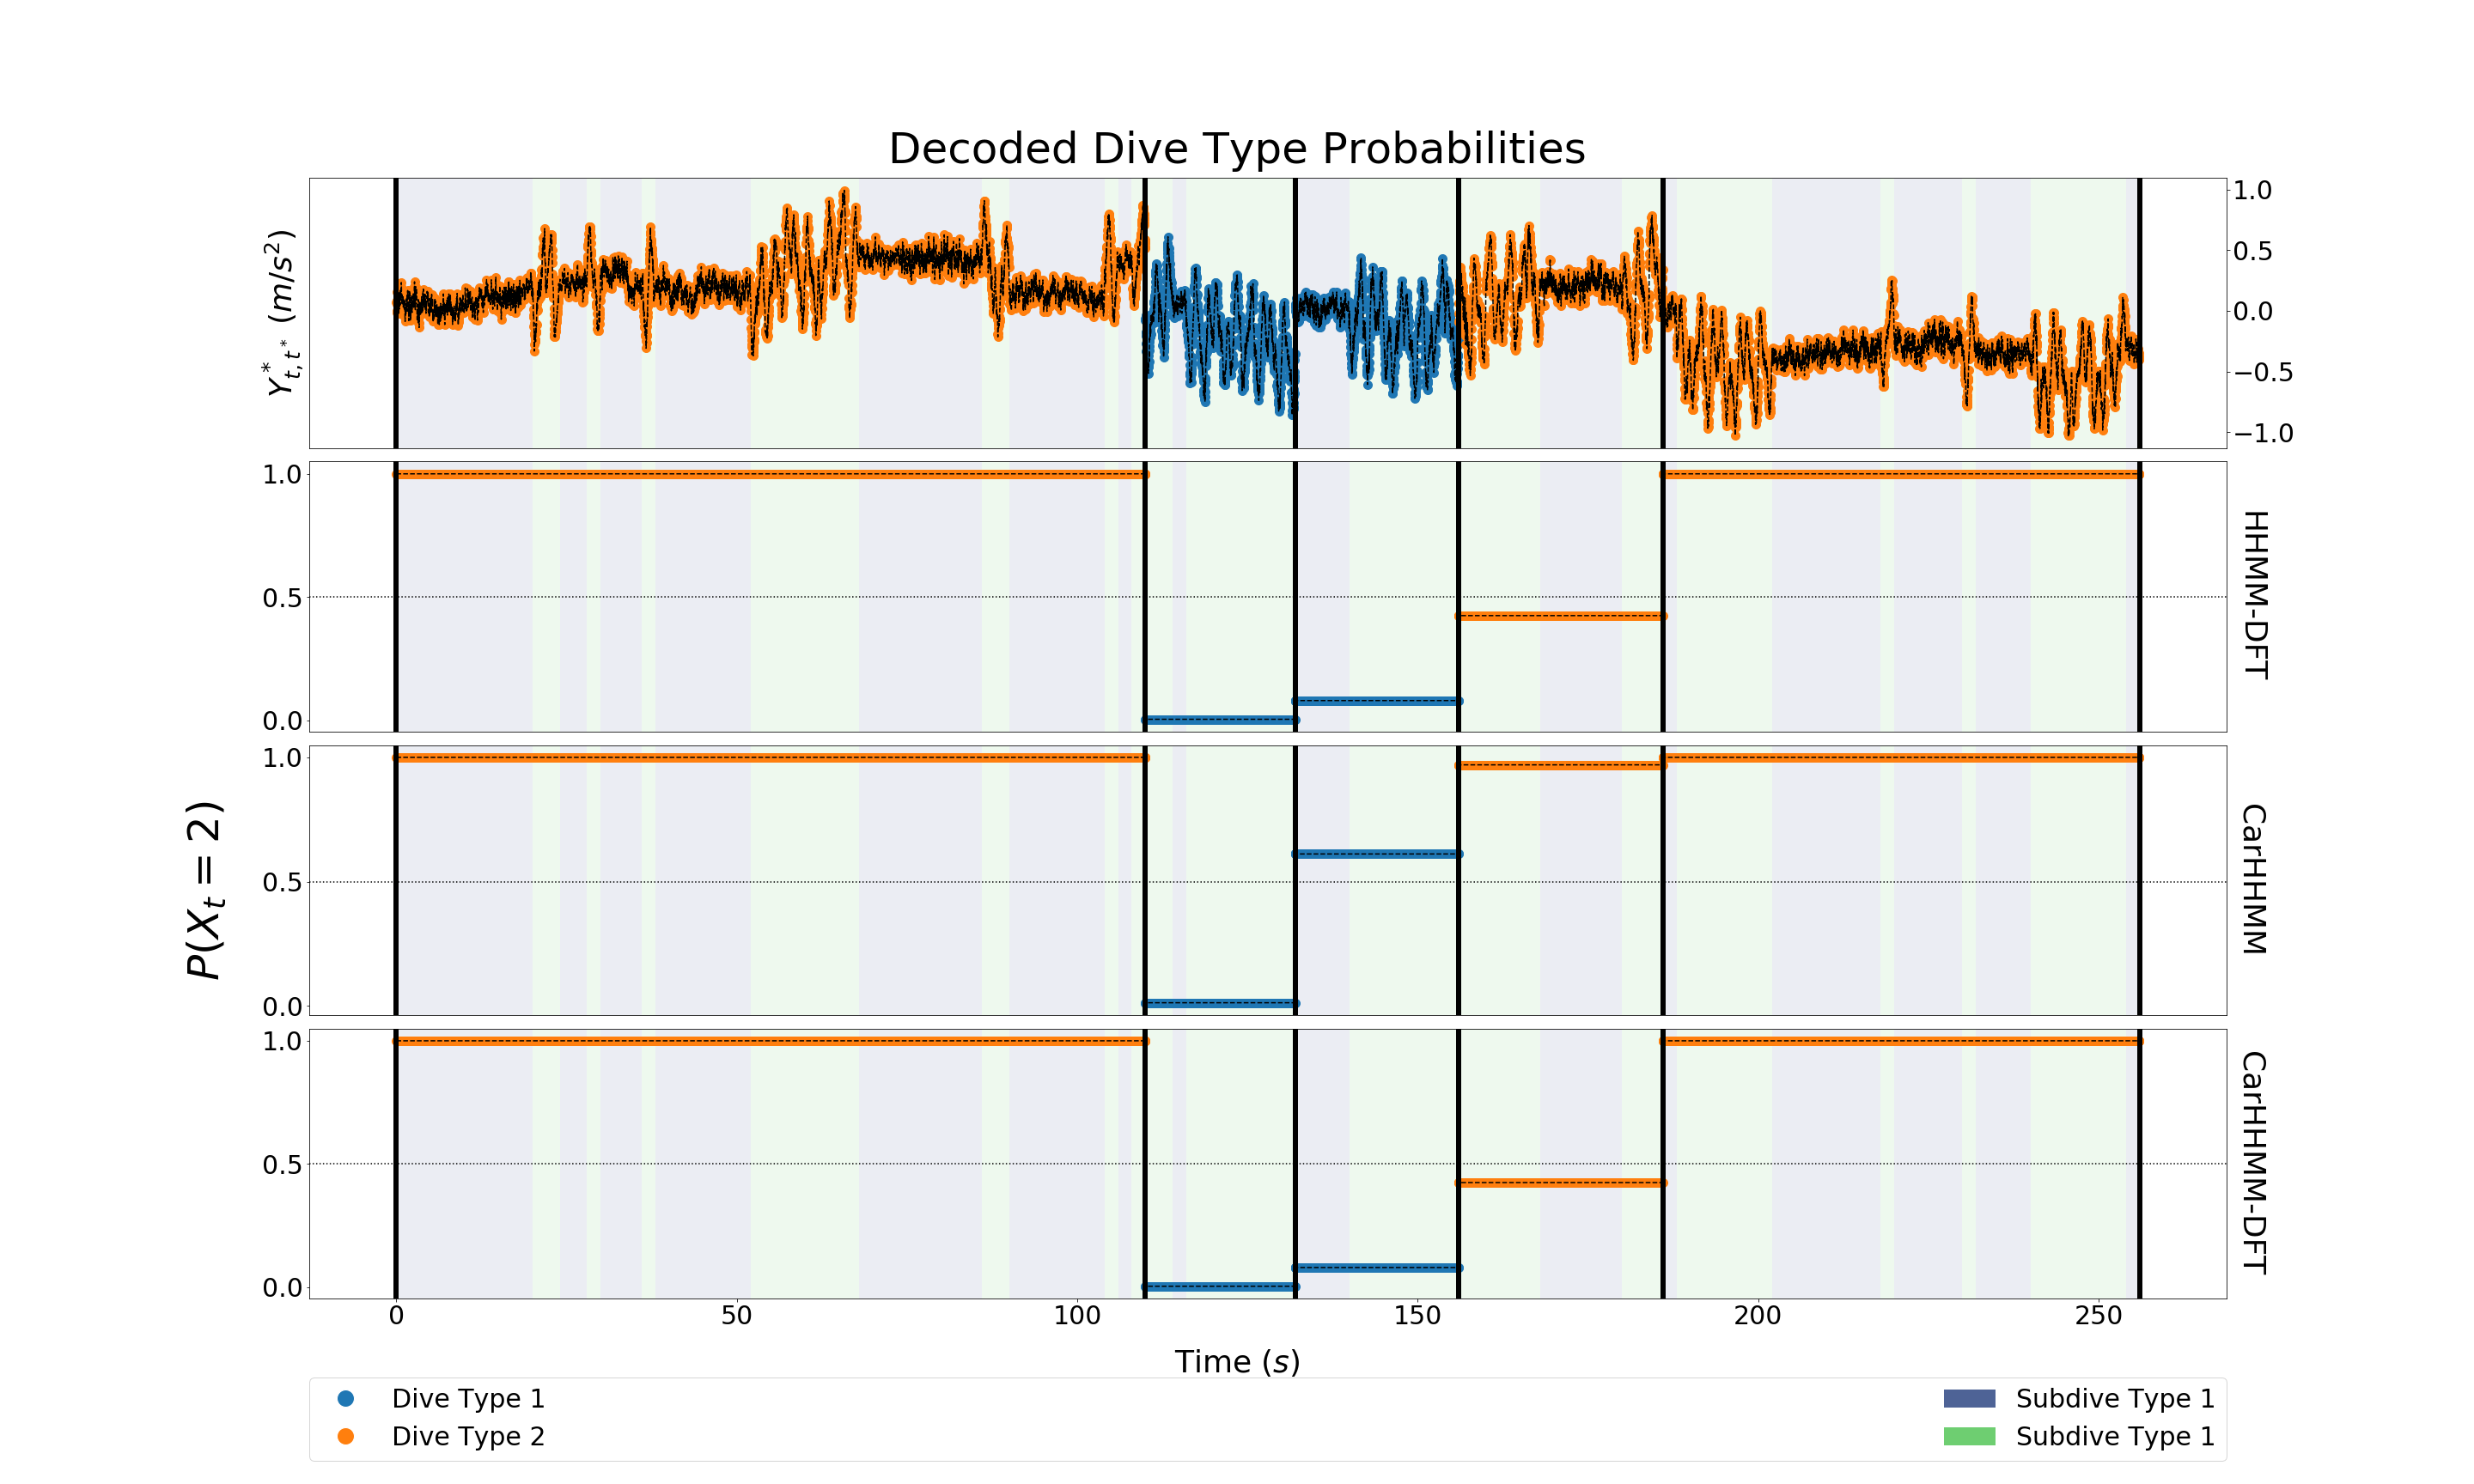
\includegraphics[width=5in]{../Plots/Posterior_Coarse_States.png}
        \caption{Coarse-scale hidden process}
    \end{subfigure}
    \newline
    \begin{subfigure}[t]{1.0\textwidth}
        \centering
        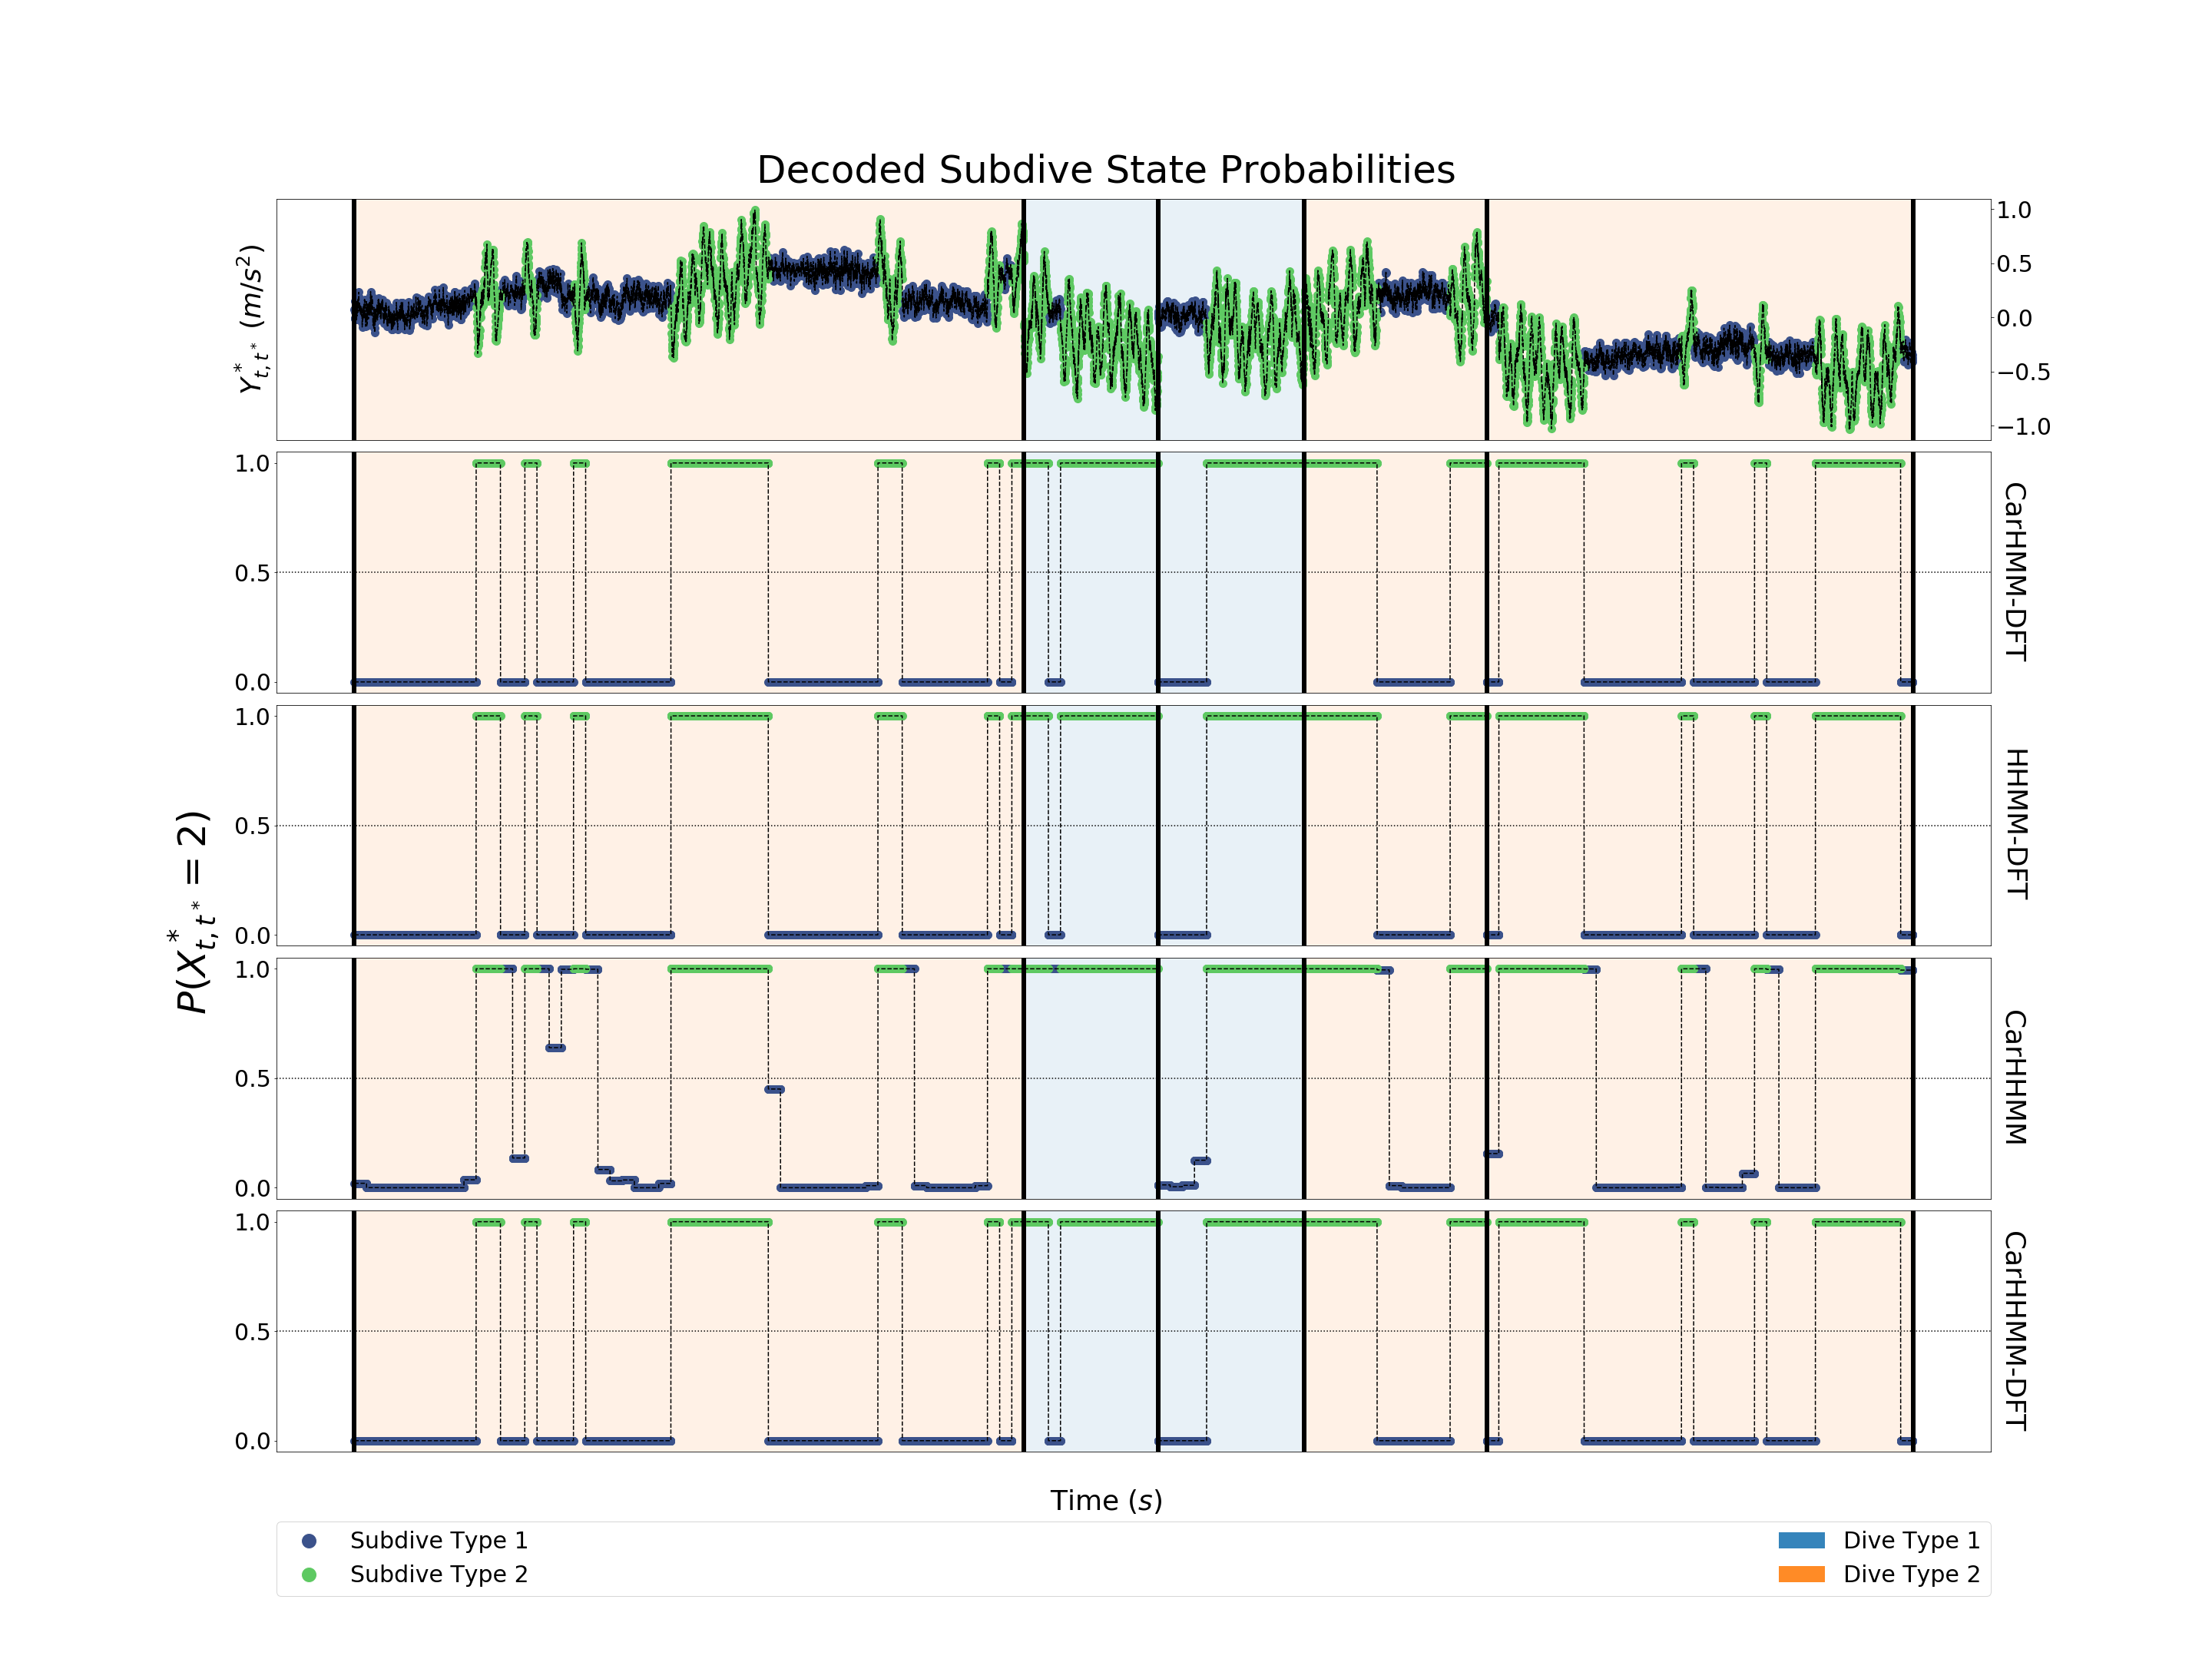
\includegraphics[width=5in]{../Plots/Posterior_Fine_States.png}
        \caption{Fine-scale hidden process}
    \end{subfigure}
	\caption{Decoded state probabilities of each model for 5 dives of one simulated data set. The colors correspond to the true behavioral state.}
	\label{fig:acc}
\end{figure}

%%% Case Study %%%

\begin{figure}[ht]
	\centering
	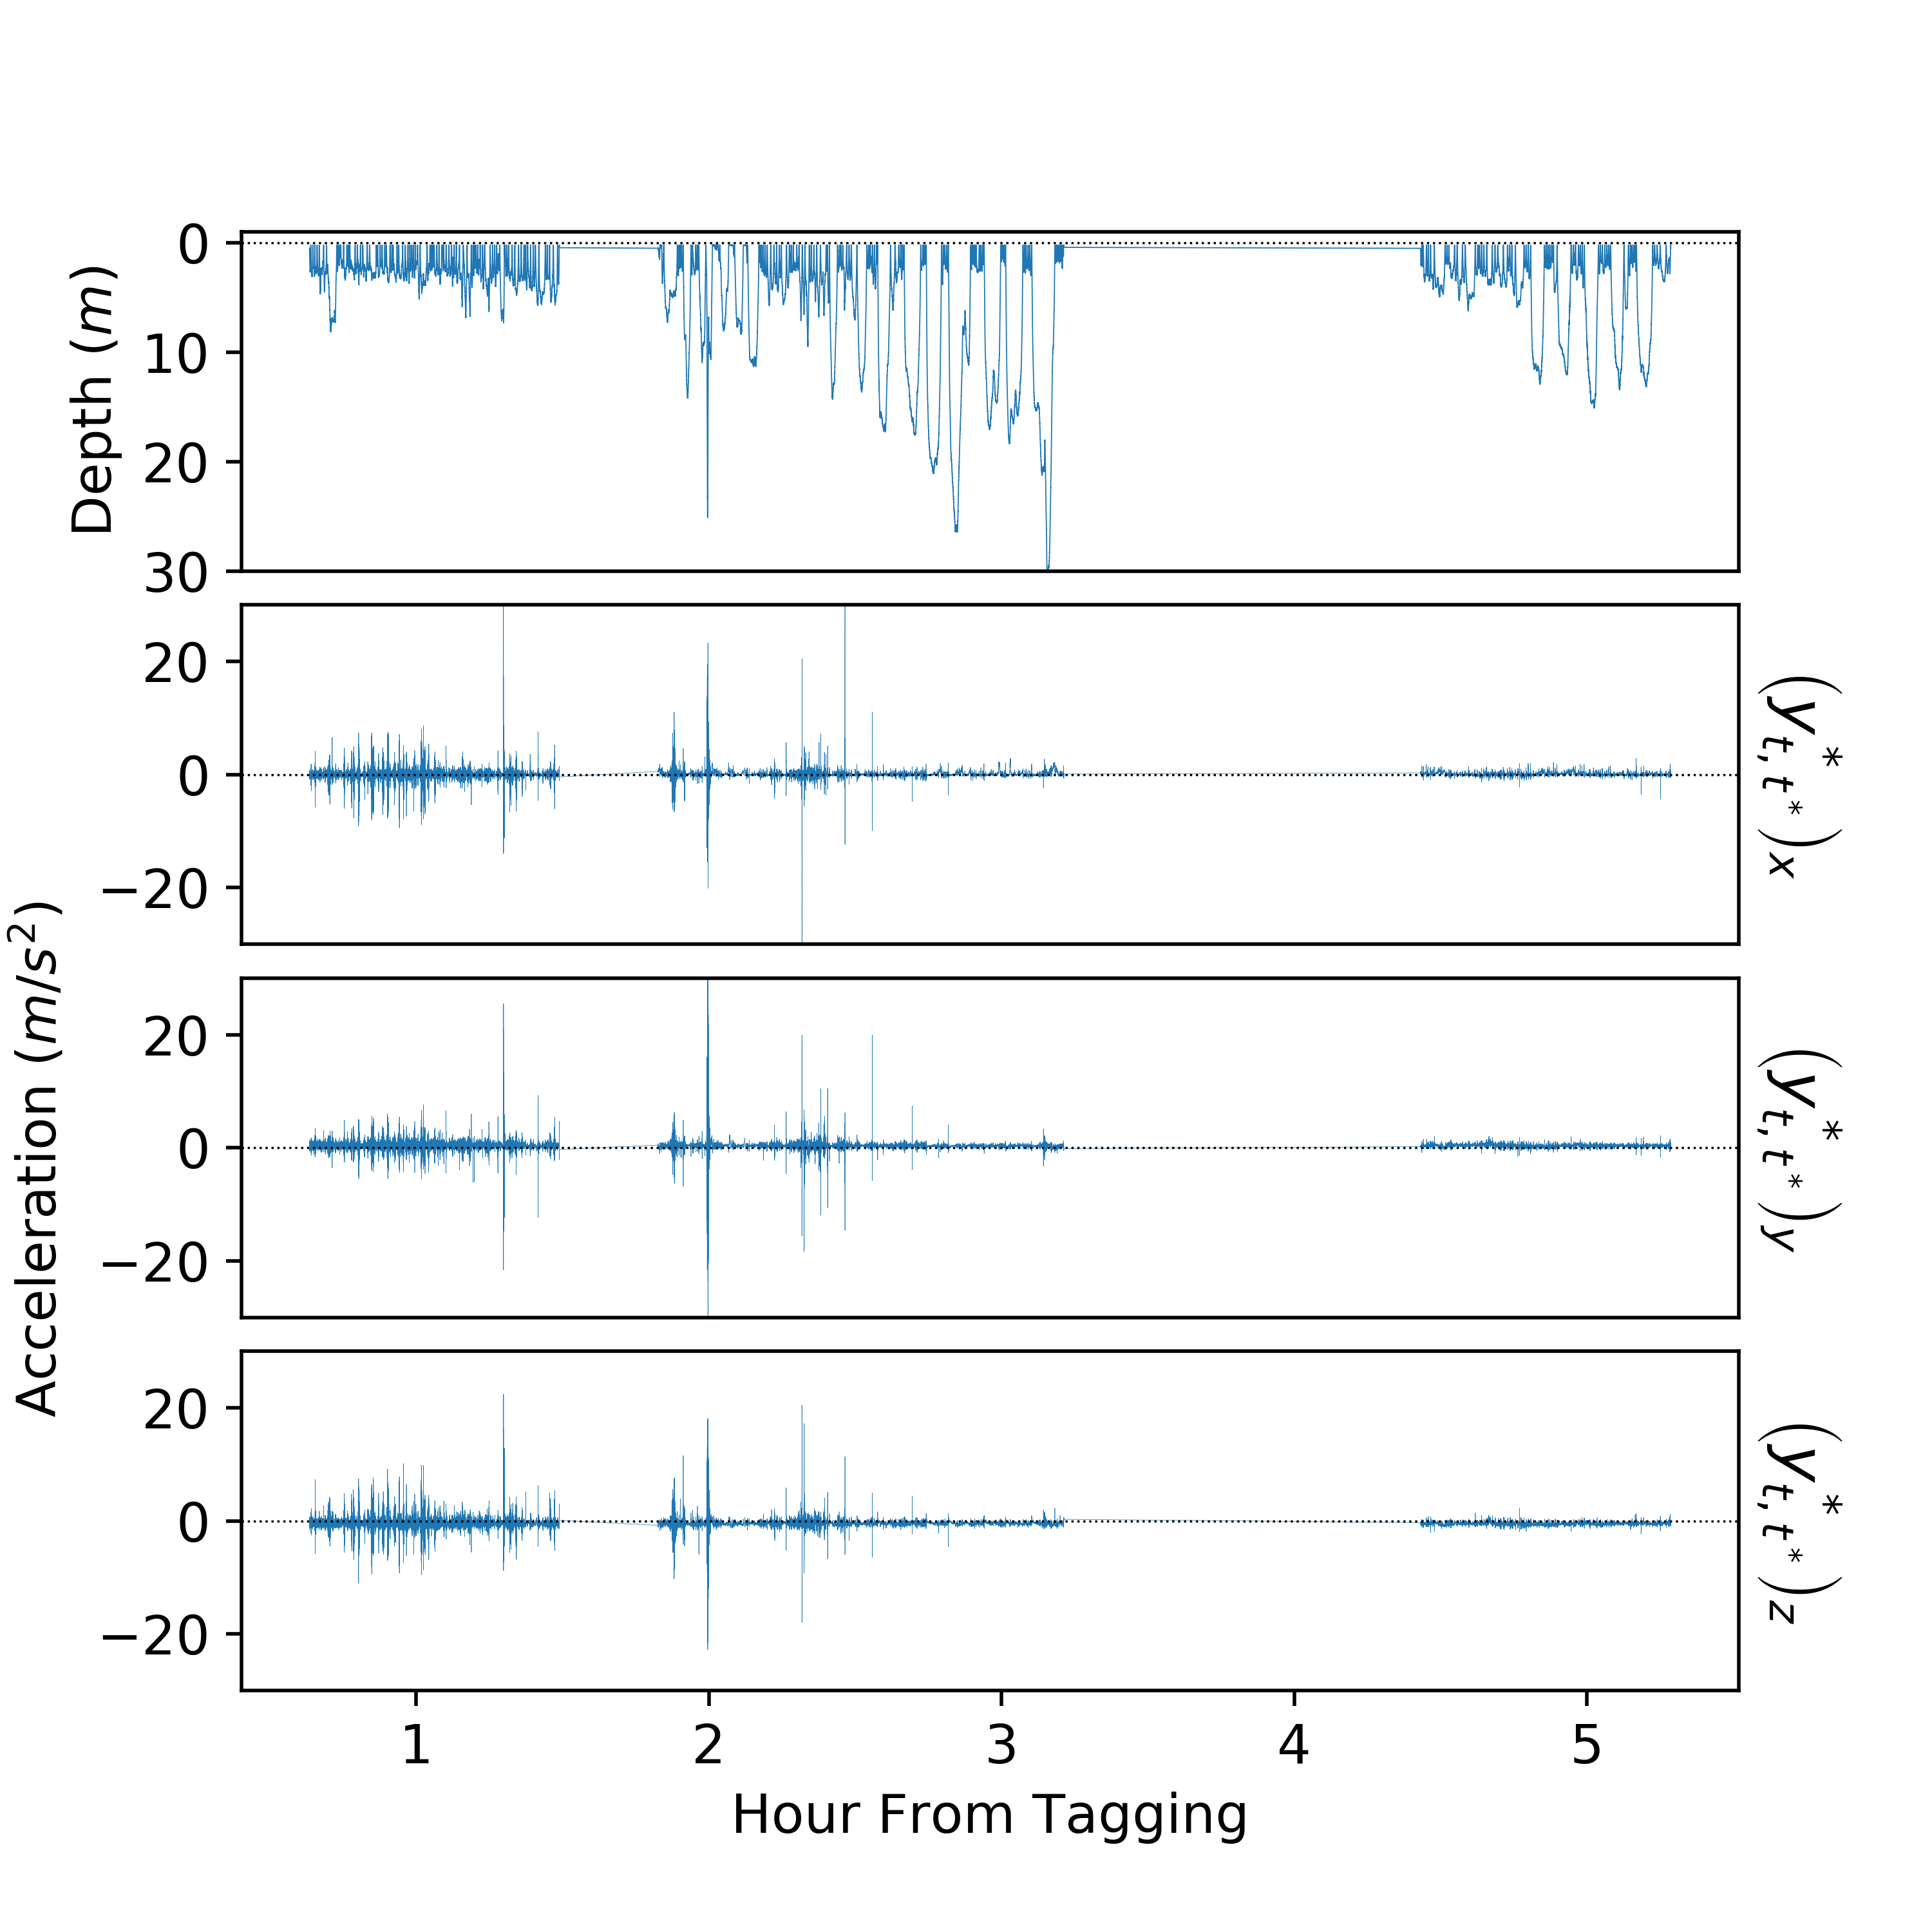
\includegraphics[width=5in]{../Plots/raw_data.png}
	\caption{Dive depth (top panel) and acceleration (bottom three panels) as functions of time, from the killer whale data set}
	\label{fig:data}
\end{figure}

\begin{figure}[ht]
	\centering
	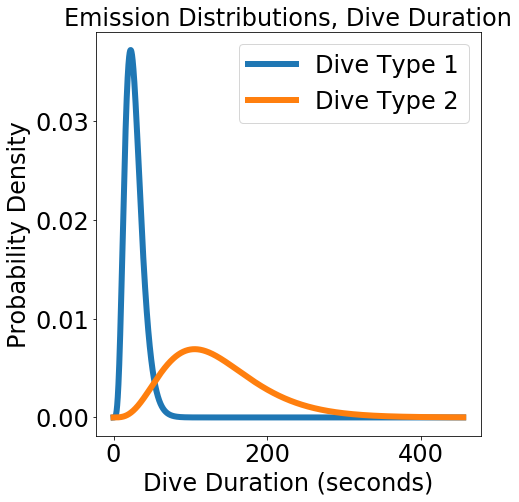
\includegraphics[width=5in]{../Plots/coarse-emissions.png}
	\caption{Estimated probability distributions for each coarse-scale observation in each dive type.}
	\label{fig:coarse_emis}
\end{figure}

\begin{figure}[ht]
	\centering
	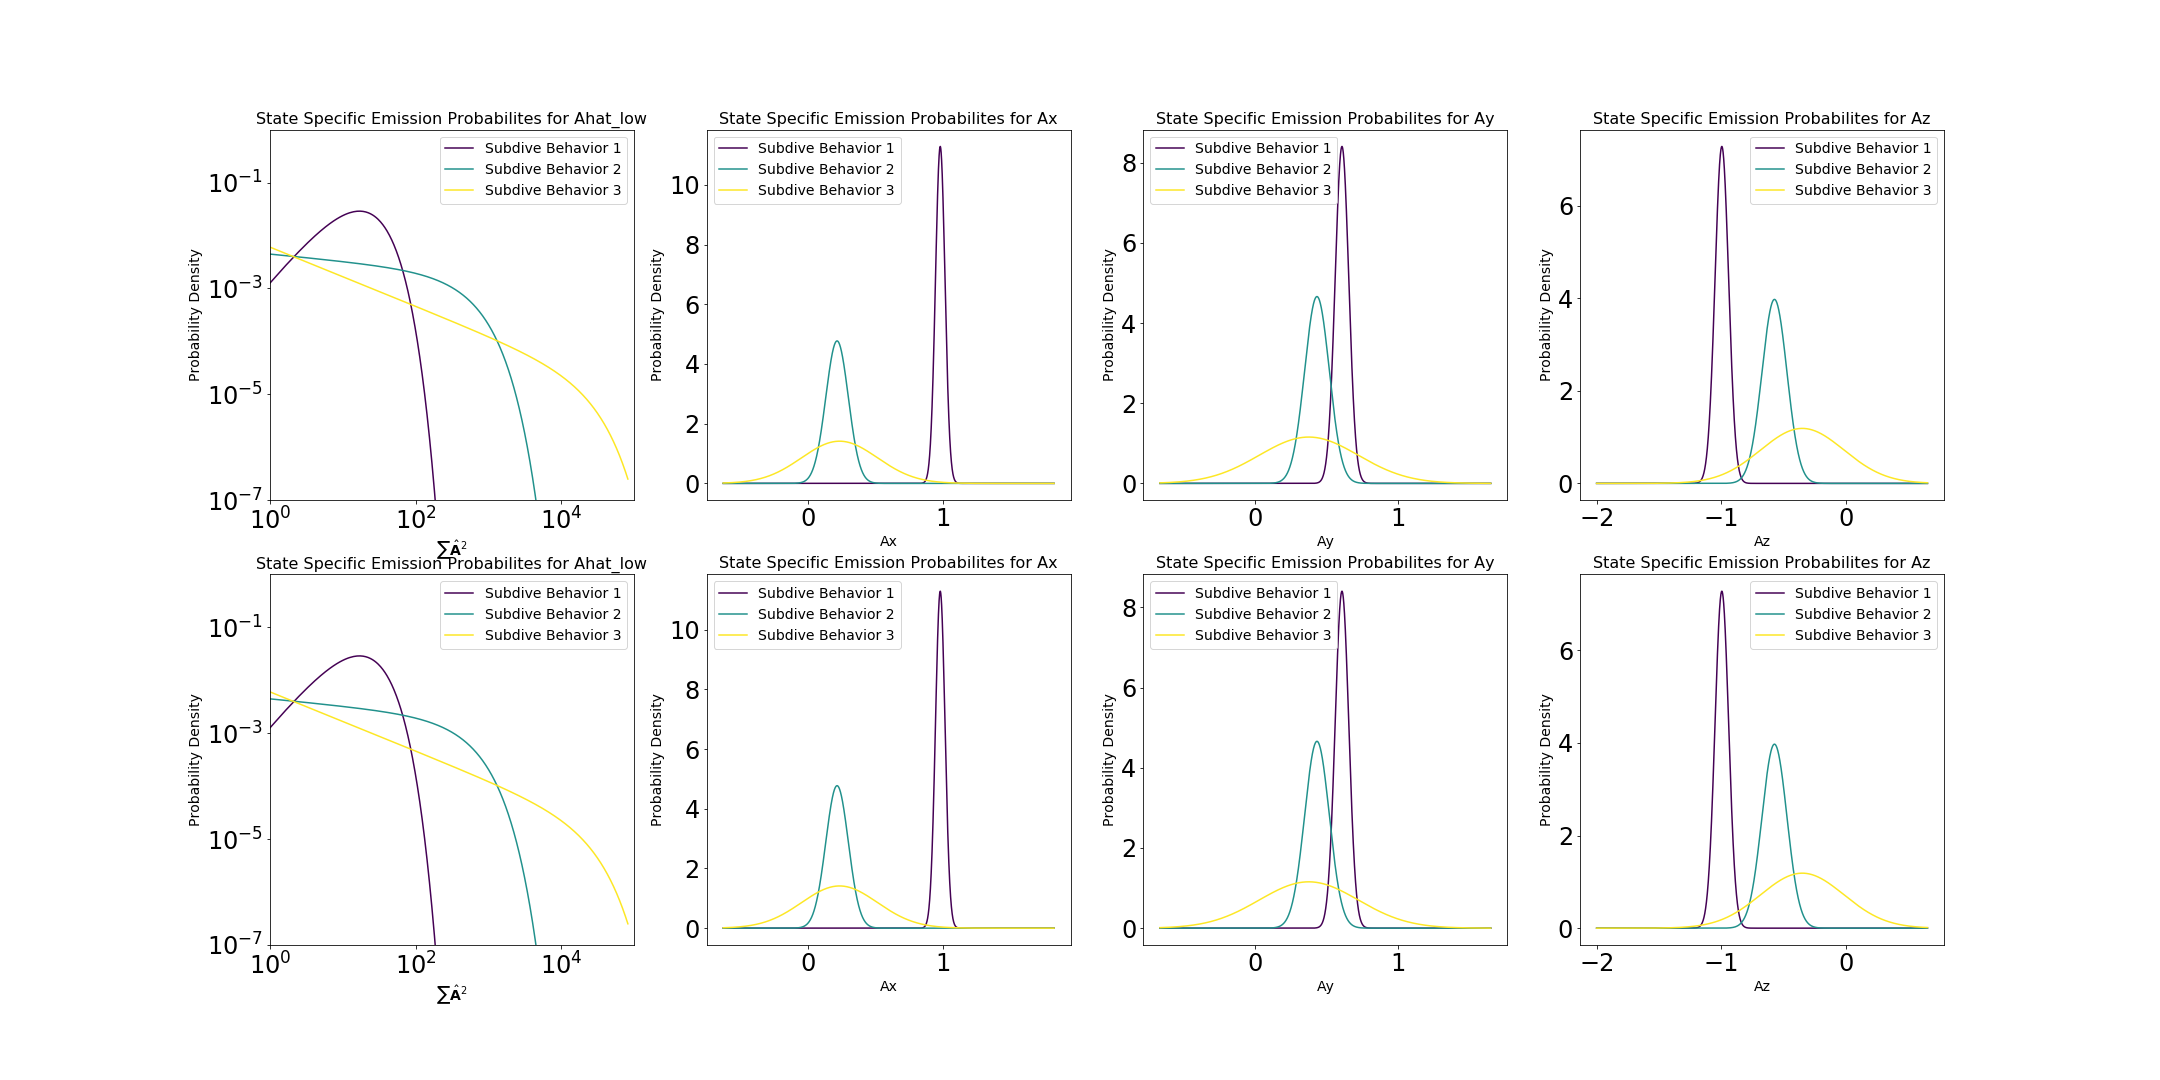
\includegraphics[width=5in]{../Plots/fine-emissions.png}
	\caption{Estimated probability distributions for each fine-scale observation in each behavioral state. Note that the distributions of acceleration do not take auto-correlation into account (see table \ref{table:emis_dists})}
	\label{fig:fine_emis}
\end{figure}

\begin{figure}[ht]
	\centering
	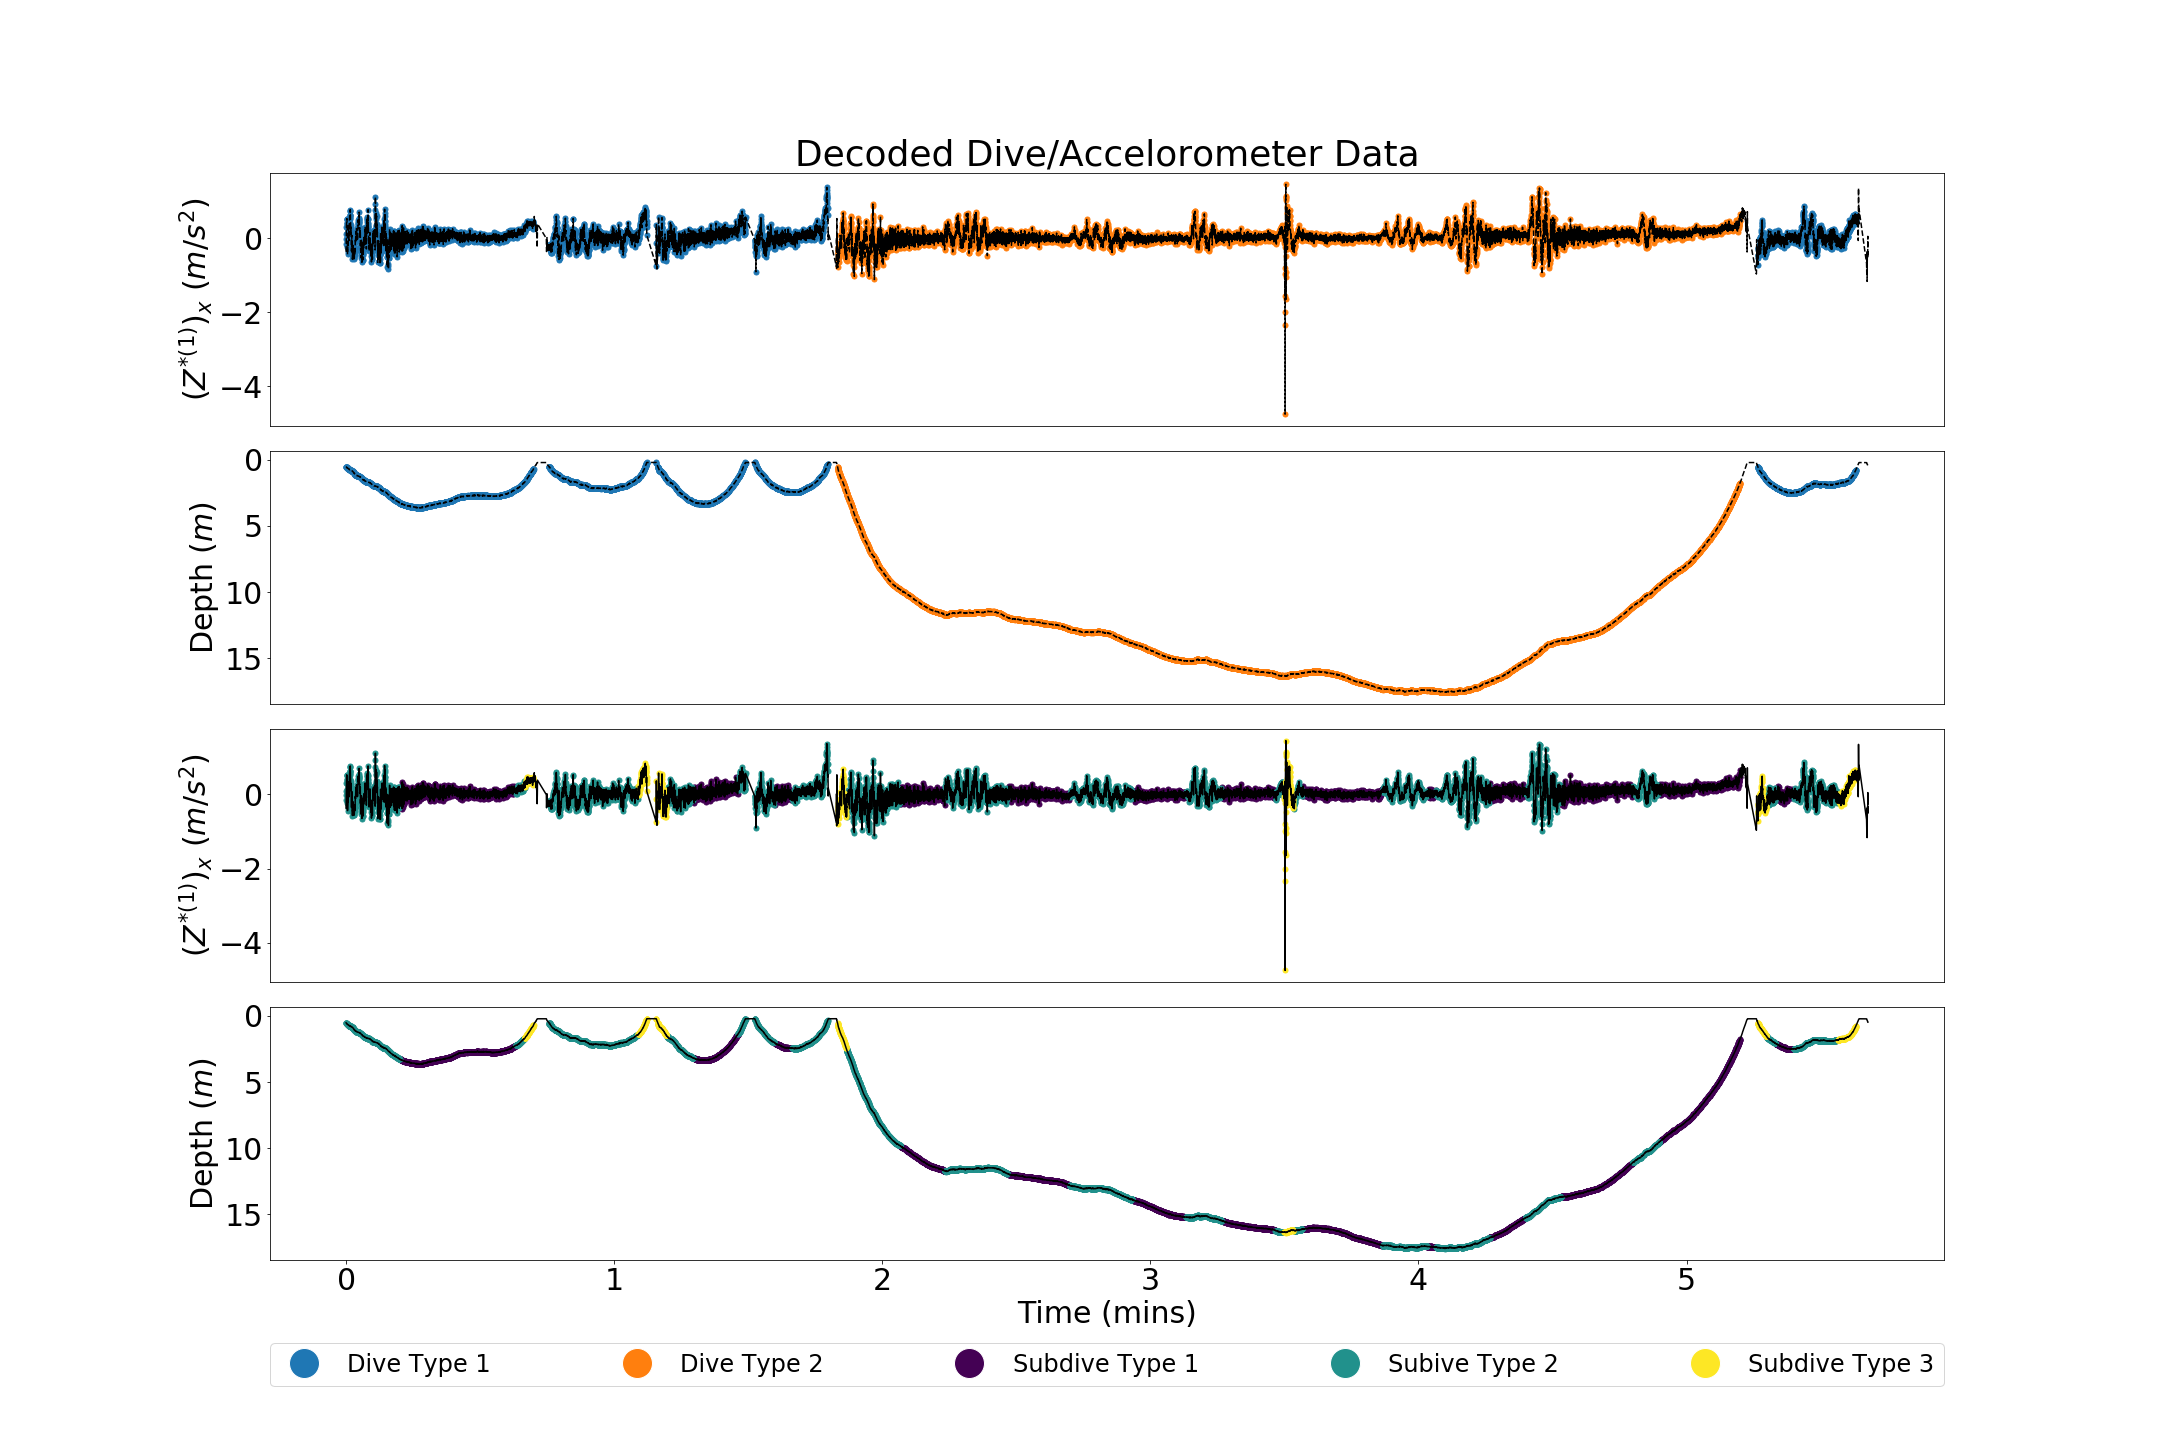
\includegraphics[width=5in]{../Plots/decoded_data.png}
	\caption{Features of a particular set of killer whale dives and decoded estimates for the intra-dive behavioral states. The color of the plot corresponds to behavioral or dive state with the highest probability.}
	\label{fig:labeled_dives}
\end{figure}

\begin{figure}[ht]
    \begin{subfigure}{0.45\textwidth}
    	\centering
    	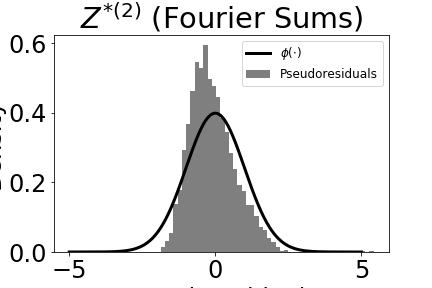
\includegraphics[width=2.25in]{../Plots/psedoresids_ahat.png}
    	\caption{Pseudoresiduals of $Z^{*(2)}$}
    	\label{fig:pseudoresids}
    \end{subfigure}
    \begin{subfigure}{0.45\textwidth}
    	\centering
    	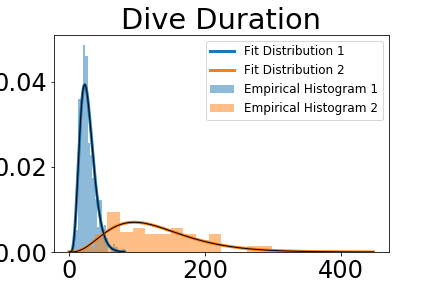
\includegraphics[width=2.25in]{../Plots/empirical_hist_dive_duration.png}
    	\caption{Empirical distribution of $Y$ (Dive Duration)}
    	\label{fig:empirical_dist}
    \end{subfigure}
    \caption{Examples of psuedoresiduals and a weighted empirical distribution as a model checking tool.}
    \label{fig:model_checking}
\end{figure}